%%%%%%%%%%%%%%%%%%%%%%%%%%%%%%%%%%%%%%%%%%%%%%%%%%%%%%%
% Please note that whilst this template provides a 
% preview of the typeset manuscript for submission, it 
% will not necessarily be the final publication layout.
%
% letterpaper/a4paper: US/UK paper size toggle
% num-refs/alpha-refs: numeric/author-year citation and bibliography toggle

%\documentclass[letterpaper]{oup-contemporary}
\documentclass[a4paper,num-refs]{oup-contemporary}

%%% Journal toggle; only specific options recognised.
%%% (Only "gigascience" and "general" are implemented now. Support for other journals is planned.)
\journal{gigascience}

\usepackage{graphicx}
\usepackage{siunitx}
\usepackage{amsmath}
\usepackage{algorithm}
\usepackage{algpseudocode}
\algnewcommand{\Inputs}[1]{%
  \State \textbf{Inputs:}
  \Statex \hspace*{\algorithmicindent}\parbox[t]{.8\linewidth}{\raggedright #1}
}
\renewcommand{\algorithmicrequire}{\textbf{Input:}}
\renewcommand{\algorithmicensure}{\textbf{Output:}}

%%% Flushend: You can add this package to automatically balance the final page, but if things go awry (e.g. section contents appearing out-of-order or entire blocks or paragraphs are coloured), remove it!
% \usepackage{flushend}

\title{Smash++: finding rearrangements}

%%% Use the \authfn to add symbols for additional footnotes, if any. 1 is reserved for correspondence emails; then continuing with 2 etc for contributions.
\author[1,\authfn{1}]{Morteza Hosseini}
\author[2,\authfn{1}]{Diogo Pratas}
\author[2,\authfn{1}]{Armando J. Pinho}

\affil[1,2]{IEETA/DETI, University of Aveiro, Portugal}

%%% Author Notes
\authnote{\authfn{1}seyedmorteza@ua.pt; pratas@ua.pt; ap@ua.pt}

%%% Paper category
\papercat{Technical note}

%%% "Short" author for running page header
\runningauthor{Hosseini et al.}

%%% Should only be set by an editor
\jvolume{00}
\jnumber{0}
\jyear{2017}

\begin{document}

\begin{frontmatter}
\maketitle
\begin{abstract}
The Abstract (250 words maximum) should be structured to include the following details: \textbf{Background}, the context and purpose of the study; \textbf{Results}, the main findings; \textbf{Conclusions}, brief summary and potential implications. Please minimize the use of abbreviations and do not cite references in the abstract.
\end{abstract}

\begin{keywords}
Keyword1; keyword 2; keyword 3 (Three to ten keywords representing the main content of the article)
\end{keywords}
\end{frontmatter}

%%% Key points will be printed at top of second page
\begin{keypoints*}
\begin{itemize}
\item This is the first point
\item This is the second point
\item One last point.
\end{itemize}
\end{keypoints*}

\section{Introduction to this Template}

\begin{epigraph}{Epigraph source name}
This is the epigraph text, should you like to add one. Lorem ipsum dolor sit amet, consectetur adipiscing elit, sed do eiusmod tempor incididunt ut labore et dolore magna aliqua. 
\end{epigraph}

This is the \LaTeX{} template for GigaScience journal manuscript submissions. \textbf{Please note that whilst this template provides a preview of the typeset manuscript for submission, it will not necessarily be the final publication layout.}

There are important commands in the preamble that you will need to modify for your own manuscript. If you are using this template on Overleaf, please switch the editor to Source code mode to view them; or if you prefer to stay in the Rich Text view, click on the title in the Rich Text view to display the preamble code.

Use the \verb|\journal{...}| command in the preamble so that the correct journal name, logo and colours are loaded automatically. \textbf{Only certain journals and options are supported at this time;} check with your journal's editorial office if your journal is supported.

Alternatively you can re-define \verb|\jname|, \verb|\jlogo| and the \verb|jcolour| explicitly, though check with your journal's editorial office to confirm that this is appropriate.

Specify your manuscript's category with the \verb|\papercat{...}| command in the preamble.

See the sample code in the preamble for a sample of how author and affiliation information can be specified.

Use later sections starting with `Background' on page~\pageref{sec:background} to write your manuscript. The remainder of this current section will provide some sample \LaTeX{} code for various elements you may want to include in your manuscript.

\subsection{Sectional Headings}
You can use \verb|\section{...}|, \verb|\subsection{...}| commands to add more sections and subsections to your manuscript. Further sectional levels are provided by \verb|\subsubsection|, \verb|\paragraph| and \verb|\subparagraph|.

\subsection{Citations and References}
Use the \verb|num-refs| document class option for numerical citations, and \verb|alph-refs| option for author-year citations.
Use the \verb|\citep| command for parenthetical citations, and \verb|\citet| command for text citations (when using \verb|alpha-refs|).
This is a citation: \citep{Fan:2004} and here are two more: \citep{Cox:1972,Hear:Holm:Step:quan:2006}.

% \begin{quote}
% This is a quote. Lorem ipsum dolor sit amet, consectetur adipiscing elit, sed do eiusmod tempor incididunt ut labore et dolore magna aliqua. Ut enim ad minim veniam, quis nostrud exercitation ullamco laboris nisi ut aliquip ex ea commodo consequat. 
% \end{quote}

\begin{itemize}
\item This is a bullet list.
\item Another point.
\item A third point.
\end{itemize}

This\footnote{This is the footnote text. This is the footnote text. This is the footnote text. This is the footnote text. This is the footnote text.} is a footnote. Lorem ipsum dolor sit amet, consectetur adipiscing elit, sed do eiusmod tempor incididunt ut labore et dolore magna aliqua.

\begin{itemize}
\item This is a numbered list.
\item Another point.
\item A third point.
\end{itemize}

Lorem ipsum dolor sit amet, consectetur adipiscing elit, sed do eiusmod tempor incididunt ut labore et dolore magna aliqua. Lorem ipsum dolor sit amet, consectetur adipiscing elit, sed do eiusmod tempor incididunt ut labore et dolore magna aliqua.


\subsubsection{This is a 3rd level heading}

Use \verb|\subsubsection| to get a 3rd level heading.
Lorem ipsum dolor sit amet, consectetur adipiscing elit, sed do eiusmod tempor incididunt ut labore et dolore magna aliqua. Lorem ipsum dolor sit amet, consectetur adipiscing elit, sed do eiusmod tempor incididunt ut labore et dolore magna aliqua. 


\paragraph{This is a 4th level heading}

Use \verb|\paragraph| to get a 4th level heading.
Lorem ipsum dolor sit amet, consectetur adipiscing elit, sed do eiusmod tempor incididunt ut labore et dolore magna aliqua. Lorem ipsum dolor sit amet, consectetur adipiscing elit. 

\subparagraph{This is a 5th level heading}

Use \verb|\subparagraph| to get a 5th level heading.
Lorem ipsum dolor sit amet, consectetur adipiscing elit, sed do eiusmod tempor incididunt ut labore et dolore magna aliqua. Lorem ipsum dolor sit amet, consectetur adipiscing elit.


\subsection{Figures and Tables}
Figures and tables can be added with the usual \verb|figure| and \verb|table| environments, e.g.~Figure \ref{fig:example} and Table \ref{tab:example}. Use \verb|figure*| and \verb|table*| if you need a two-column wide figure or table, as in Figure \ref{fig:example:wide} and Table \ref{tab:example:wide}. 

If you have a very wide table or figure, you can use \texttt{sidewaystable} or \texttt{sidewaysfigure}, as in Table \ref{tab:example:sideways}: this will be rotated sideways and occupy a \emph{single column} on its own.

If your table or figure is both wide and tall (so it wouldn't fit well in a single column with \texttt{sidewaystable} or \texttt{figure}), 
you can use \verb|table| or \verb|figure| inside a \verb|landscape| environment for a full-page landscaped alternative. A page break will be inserted \emph{immediately before and after} the \verb|landscape| environment (Table \ref{tab:example:landscape}), so you'll need to carefully position it in a suitable location in your manuscript.

% \begin{figure}[bt!] %% preferably at bottom or top of column
% \centering
% 
\includegraphics[width=\linewidth]{example-image}
% \caption{An example figure}\label{fig:example}
% \end{figure}

% \begin{table}[bt!]
% \caption{An example table.}\label{tab:example}
% \begin{tabular}{l r l}
% \toprule
% Item & Quantity & Notes\\
% \midrule
% Widgets & 42 & Over-supplied\textsuperscript{*} \\
% Gadgets & 13 & Under-supplied \\
% \bottomrule
% \end{tabular}
% \begin{tablenotes}
% \item This is a table note.
% \item \textsuperscript{*}Another note.
% \end{tablenotes}
% \end{table}


\subsection{Some Mathematics Sample}

Let $X_1, X_2, \ldots, X_n$ be a sequence of independent and identically distributed random variables with $\text{E}[X_i] = \mu$ and $\text{Var}[X_i] = \sigma^2 < \infty$, and let
%
\begin{equation}
S_n = \frac{X_1 + X_2 + \cdots + X_n}{n}
      = \frac{1}{n}\sum_{i}^{n} X_i
\end{equation}
%
denote their mean. Then as $n$ approaches infinity, the random variables $\sqrt{n}(S_n - \mu)$ converge in distribution to a normal $\mathcal{N}(0, \sigma^2)$.


\section{Background}
\label{sec:background}

The background section should be written in a way that is accessible to researchers without specialist knowledge in that area and must clearly state---and, if helpful, illustrate---the background to the research and its aims. The section should end with a brief statement of what is being reported in the article.


\section{Data Description}

A statement providing background and purpose for collection of these data should be presented for readers without specialist knowledge in that area. A brief description of the protocol for data collection, data curation and quality control, as well as potential uses should be included, as well as outlining how the data can be accessed if it is not deposited in our repository.

% \begin{figure*}%[b!]  %% Add a [b!] if you prefer the wide image to be at the bottm of the page
% \centering
% 
\includegraphics[width=.7\textwidth]{example-image}
% \caption{An example wide figure. Lorem ipsum dolor sit amet, consectetur adipiscing elit, sed do eiusmod tempor incididunt ut labore et dolore magna aliqua.
% }\label{fig:example:wide}
% \end{figure*}


\section{Analyses}

This section should provide details of all of the experiments and analyses that are required to support the conclusions of the paper. The authors should make clear the goal of each analysis and state the basic findings.


% \begin{table*}[bt!]
% \caption{Automobile land speed records (GR 5-10)}\label{tab:example:wide}
% % Use "S" column identifier (from siunitx) to align on decimal point.
% % Use "L", "R" or "C" column identifier for auto-wrapping columns with tabularx.
% \begin{tabularx}{\linewidth}{S l l l r L}
% \toprule
% {Speed (mph)} & {Driver} & {Car} & {Engine} & {Date} & {Extra comments}\\
% \midrule
% 407.447     & Craig Breedlove & Spirit of America          & GE J47    & 8/5/63  & (Just to demo a full-width table with auto-wrapping long lines) \\
% 413.199     & Tom Green       & Wingfoot Express           & WE J46    & 10/2/64  \\
% 434.22      & Art Arfons      & Green Monster              & GE J79    & 10/5/64  \\
% 468.719     & Craig Breedlove & Spirit of America          & GE J79    & 10/13/64 \\
% 526.277     & Craig Breedlove & Spirit of America          & GE J79    & 10/15/65 \\
% 536.712     & Art Arfons      & Green Monster              & GE J79    & 10/27/65 \\
% 555.127     & Craig Breedlove & Spirit of America, Sonic 1 & GE J79    & 11/2/65  \\
% 576.553     & Art Arfons      & Green Monster              & GE J79    & 11/7/65  \\
% 600.601     & Craig Breedlove & Spirit of America, Sonic 1 & GE J79    & 11/15/65 \\
% 622.407     & Gary Gabelich   & Blue Flame                 & Rocket    & 10/23/70 \\
% 633.468     & Richard Noble   & Thrust 2                   & RR RG 146 & 10/4/83  \\
% 763.035     & Andy Green      & Thrust SSC                 & RR Spey   & 10/15/97\\
% \bottomrule
% \end{tabularx}
%
% \begin{tablenotes}
% \item Source is from this website: \url{https://www.sedl.org/afterschool/toolkits/science/pdf/ast_sci_data_tables_sample.pdf}
% \end{tablenotes}
% \end{table*}


\section{Discussion}

The discussion should spell out the major conclusions and interpretations of the work, including some explanation on the importance and relevance of the dataset and analysis. It should not be restatement of the analyses done and their basic conclusions. The discussion section can end with a concluding paragraph that clearly states the main conclusions of the research along with directions for future work. Summary illustrations can be included.

% \begin{sidewaystable}
% \caption{Automobile land speed records (GR 5-10). This is the same table as before, but rotated sideways.}
% \label{tab:example:sideways}
% % Use "S" column identifier (from siunitx) to align on decimal point.
% % Use "L", "R" or "C" column identifier for auto-wrapping columns with tabularx.
% \begin{tabularx}{\linewidth}{S l l l r L}
% \toprule
% {Speed (mph)} & {Driver} & {Car} & {Engine} & {Date} & {Extra comments}\\
% \midrule
% 407.447     & Craig Breedlove & Spirit of America          & GE J47    & 8/5/63  & (Just to demo a full-width table with auto-wrapping long lines) \\
% 413.199     & Tom Green       & Wingfoot Express           & WE J46    & 10/2/64  \\
% 434.22      & Art Arfons      & Green Monster              & GE J79    & 10/5/64  \\
% 468.719     & Craig Breedlove & Spirit of America          & GE J79    & 10/13/64 \\
% 526.277     & Craig Breedlove & Spirit of America          & GE J79    & 10/15/65 \\
% 536.712     & Art Arfons      & Green Monster              & GE J79    & 10/27/65 \\
% 555.127     & Craig Breedlove & Spirit of America, Sonic 1 & GE J79    & 11/2/65  \\
% 576.553     & Art Arfons      & Green Monster              & GE J79    & 11/7/65  \\
% 600.601     & Craig Breedlove & Spirit of America, Sonic 1 & GE J79    & 11/15/65 \\
% 622.407     & Gary Gabelich   & Blue Flame                 & Rocket    & 10/23/70 \\
% 633.468     & Richard Noble   & Thrust 2                   & RR RG 146 & 10/4/83  \\
% 763.035     & Andy Green      & Thrust SSC                 & RR Spey   & 10/15/97\\
% \bottomrule
% \end{tabularx}

% \begin{tablenotes}
% \item Source is from this website: \url{https://www.sedl.org/afterschool/toolkits/science/pdf/ast_sci_data_tables_sample.pdf}
% \end{tablenotes}
% \end{sidewaystable}


\section{Potential implications}

Authors should provide some additional comments about potential, more broad-ranging implications of their work that are not directly related to the current focus of their manuscript. This section is meant to promote discussion on possible ways the findings or data presented might be used in or have a relationship with other areas of research that may not be directly apparent in the work. It is not meant to provide `proof of importance' of the work. Only to engender expansion of use to other areas. 

Explicit personal opinions by the authors are permitted, but they should be made clear as such. References or related information to support the propositions should be included. These section should focus on work that can be done within the foreseeable future and specifically using the information within the manuscript, not provide speculation on how it will relate to far-reaching goals of the research area.


\section{Methods} \label{sec.methods}
The schema of the proposed method is illustrated in Figure~\ref{fig.schema}. Smash++ takes as inputs a reference and a target file and produces as output a position file, which is then fed to the Smash++ visualizer to produce an SVG image. This process has eight major stages: (1)~compression of the original target file, based on the model of original reference file, (2)~filtering and segmentation of the compressed file, (3)~reference-free compression of the segmented files, obtained by the previous stage, (4)~compression of the original reference file, based on the model of segmented files obtained by stage~2, (5)~filtering and segmentation of the compressed files, (6)~reference-free compression of the segmented files, that are obtained by the stage~5, (7)~aggregating positions, generated by stages~3 and~6, and (8)~visualizing the positions. The following sections describe the process in detail.

\begin{figure*}[!t]
  \centering
  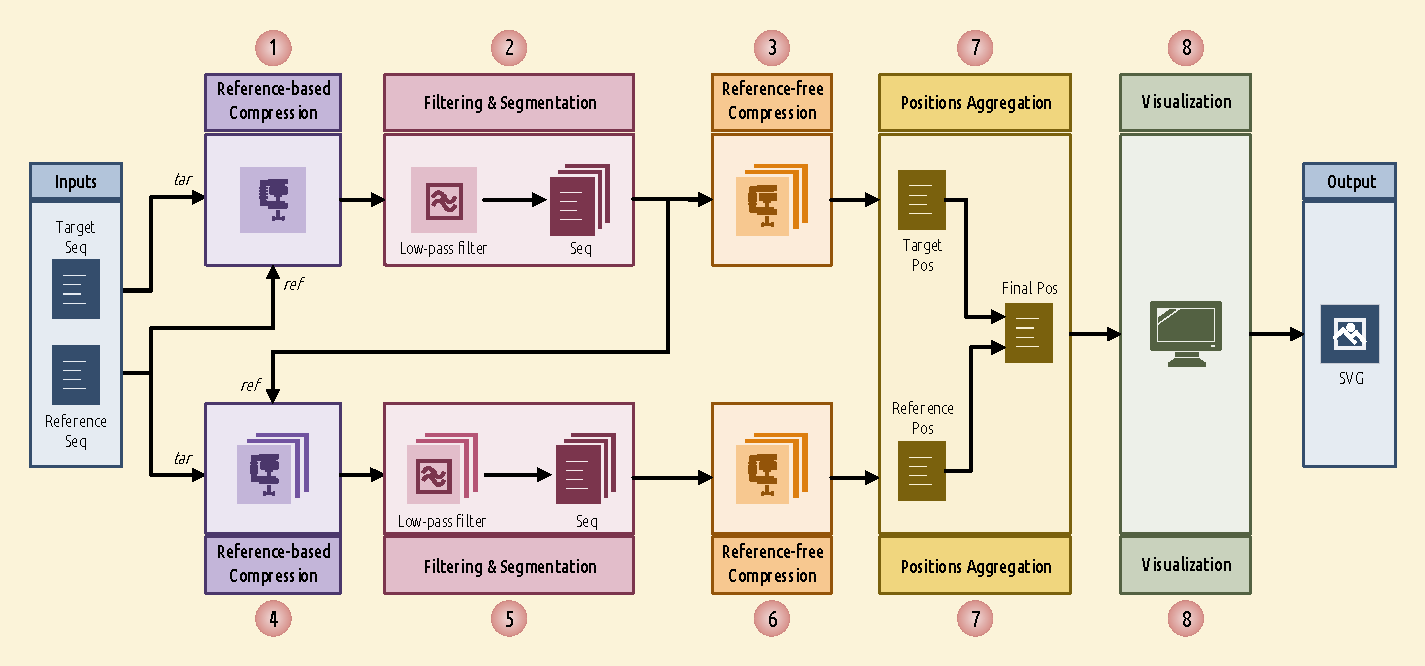
\includegraphics[width=.9\linewidth]{schema.pdf}
  \caption{The schema of Smash++. The process of finding similar regions in reference and target sequences and also, computing redundancy in each region includes eight stages. Finally, Smash++ outputs a *.pos file that includes the positions of the similar regions, and can be then visualized, resulting in an SVG image.}
  \label{fig.schema}
\end{figure*}

\subsection{Data modeling}
Smash++ works on the basis of cooperation between finite-context models (FCMs) and substitutional tolerant Markov models (STMMs). Applying these models on various contexts provides probability and weight values, illustrated in Figure~\ref{fig.model}a, which are then mixed (by multiplication and addition, shown in Figure~\ref{fig.model}b) to provide the final probability ($P$) of occurring an input symbol. The following subsections describe FCMs and STMMs in detail.

\begin{figure}[!t]
  \centering
  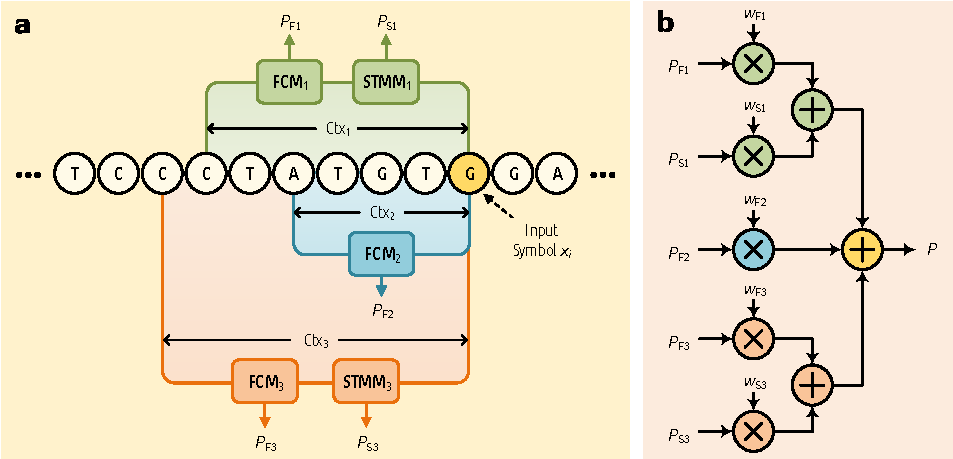
\includegraphics[width=\columnwidth]{data_model.pdf}
  \caption{Data modelling by Smash++. (a) cooperation between finite-context models (FCMs) and substitutional-tolerant Markov models (STMMs). Note that each STMM needs to be associated with an FCM. (b) probability of an input symbol is estimated by employing the probability and weight values that have been obtained from processing previous symbols.}
  \label{fig.model}
\end{figure}

\subsubsection*{Finite-context model (FCM)}
A finite-context model considers Markov property to estimate the probability of the next symbol in an information source, based on the past $k$ symbols (a context of size $k$)~\cite{sayood2017introduction,hosseini2019ac,pinho2013mfcompress}. Denoting the context as $c_{k,\,i} = s_{i-k} s_{i-k+1}\ldots s_{i-2} s_{i-1}$, the probability of the next symbol $s_i$ in an information source $S$, which is posed at $i$, can be estimated as
\begin{equation} \label{eq.estimate}
  P_m(s_i|c_{k,\,i}) = \frac{N(s_i|c_{k,\,i})+\alpha}{N(c_{k,\,i})+ \alpha|\Theta|},
\end{equation}
in which $m$ stands for model (FCM in this case), $N(s_i|c_{k,\,i})$ shows the number of times that the information source has generated symbol~$s_i$ in the past, $|\Theta|$ denotes size of the alphabet~$\Theta$, $N(c_{k,\,i}) = \sum_{b \in \Theta} N(b|c_{k,\,i})$ represents the total number of events occurred for the context~$c_{k,\,i}$ and $\alpha$ allows to keep a balance between the maximum likelihood estimator and the uniform distribution. Eq.~\ref{eq.estimate} turns to the Laplace estimator, for $\alpha=1$, and also behaves as a maximum likelihood estimator, for large number of events~$i$~\cite{pratas2015alignment}.

 \subsubsection*{Substitutional tolerant Markov model (STMM)}
 A substitutional tolerant Markov model~\cite{pratas2017substitutional} is a probabilistic-algorithmic model that assumes at each position, the next symbol in the information source is the symbol which has had the highest probability of occurrence in the past. This way, an STMM ignores the real next symbol in the source. Denoting the past $k$ symbols as $c_{k,\,i} = s_{i-k} s_{i-k+1}\ldots s_{i-2} s_{i-1}$, the probability of the next symbol $s_i$, can be estimated as
 \begin{equation}
   P_m(s_i|{c'}_{k,\,i}) = \frac{N(s_i|{c'}_{k,\,i})+\alpha}{N({c'}_{k,\,i})+ \alpha|\Theta|},
 \end{equation}
 where $N$ represents the number of occurrences of symbols, that is saved in memory, and ${c'}_{k,\,i}$ is a copy of the context $c_{k,\,i}$ which is modified as
 \begin{equation}
   {c'}_{k,\,i} = \mathop{\mathrm{arg\,max}}_{\forall b\in \Theta}{P_m(b|{c'}_{k,\,i})}.
 \end{equation}

STMMs can be used along with FCMs to modify the behavior of Smash++ in confronting with nucleotide substitutions in genomic sequences. These models have the potential to be disabled, to reduce the number of mathematical calculations and consequently, increase the performance of the proposed method. Such operation is automatically performed using an array of size $k$ (the context size), named history, which preserves the past $k$ hits/misses. Seeing a symbol in the information source, the memory is checked for the symbol with the highest number of occurrences. If they are equal, a hit is saved in the history array; otherwise, a miss is inserted into the array. Before getting to store a hit/miss in the array, it is checked for the number of misses and in the case they are more than a predefined threshold $t$, the STMM will be disabled and also the history array will be reset. This process is performed for each symbol in the sequence.

This example shows the distinction between a finite-context model and a substitutional tolerant Markov model. Assume, the current context at position $i$ is $c_{11,\,i}=\textrm{GGCTAACGTAC}$, and the number of occurrences of symbols saved in memory is $\textrm{A}=10$, $\textrm{C}=12$, $\textrm{G}=13$ and $\textrm{T}=11$. Also, the symbol to appear in the sequence is $\textrm{T}$. An FCM would consider the next context as $c_{11,\,i+1}=\textrm{GCTAACGTACT}$, while an STMM would consider it as ${c'}_{11,\,i+1}=\textrm{GCTAACGTACG}$, since the base $\textrm{G}$ is the most probable symbol, based on the number of occurrences stored in memory.

 \subsubsection*{Cooperation of FCMs and STMMs} \label{sec.coop}
 When FCMs and STMMs are in cooperation, the probability of the next symbol $s_i$ in an information source $S$, at position $i$, can be estimated as
 \begin{multline} \label{eq.coop}
   P(s_i) = \sum_{m\in M_F} P_m(s_i|c_{k,\,i})\;w_{m,\,i} + \sum_{m\in M_S} P_m(s_i|{c'}_{k,\,i})\;{w'}_{m,\,i},\\
   \forall s_i\in S,~1\le i\le |S|,~1\le k\le i-1,
 \end{multline}
 in which $M_F$ and $M_S$ denote sets of FCMs and STMMs, respectively, $P_m(s_i|c_{k,\,i})$ shows the probability of the next symbol estimated by the FCM, $P_m(s_i|{c'}_{k,\,i})$ represents this probability estimated by the STMM, and $w_{m\,i}$ and ${w'}_{m,\,i}$ are weights assigned to each model based on its performance. We have
 \begin{align}
   \forall m\in M_F: \quad & w_{m,\,i} \propto (w_{m,\,i-1})^{\gamma_m} P_m(s_i|c_{k+1,\,i-1}),
   \nonumber
   \\[1mm]
   \forall m\in M_S: \quad & {w'}_{m,\,i} \propto ({w'}_{m,\,i-1})^{{\gamma'}_m} P_m(s_i|{c'}_{k+1,\,i-1}),
 \end{align}
 where $\gamma_m$ and ${\gamma'}_m \in [0,1)$ are forgetting factors predefined for each model. Also,
 \begin{equation}
   \sum_{m\in M_F} w_{m,\,i} + \sum_{m\in M_S} {w'}_{m,\,i} = 1.
 \end{equation}
 By experimenting different forgetting factors for models, we have found that higher factors should be assigned to models that have higher context-order sizes (less complexity) and vice versa. As an example, when the context size $k=6$, $\gamma_m~\mathrm{or}~{\gamma'}_m \simeq 0.9$ and when $k=18$, $\gamma_m~\mathrm{or}~{\gamma'}_m \simeq 0.95$ would be appropriate choices. These values show that forgetting factor and complexity of a model are inversely related.

 \subsubsection*{Storing models in memory}
 The FCMs and STMMs include, in fact, count values which need to be saved in memory. For this purpose, four different data structures have been employed considering the context-order size $k$, as follows:
 \begin{itemize}
   \item table of 64 bit counters, for $k \in [1, 11]$,
   \item table of 32 bit counters, for $k=\{12, 13\}$,
   \item table of 8 bit approximate counters, for $k=14$, and
   \item Count-Min-Log sketch of 4 bit counters, for $k \ge 15$.
 \end{itemize}

%  \begin{equation*}
%    \textrm{data structure} =
%    \begin{cases}
%      \textrm{table of 64 bit counters},               & 1 \leq k \leq 11 \\
%      \textrm{table of 32 bit counters},               & k=12, 13         \\
%      \textrm{table of 8 bit approximate counters},    & k=14             \\
%      \textrm{Count-Min-Log sketch of 4 bit counters}. & k \ge 15
%    \end{cases}
%  \end{equation*}

 \begin{figure*}[!h]
   \centering
   \includegraphics[width=.8\linewidth]{data_struct.pdf}
   \caption{The data structures used by Smash++ to store the models in memory. (a) table of 64~bit counters that uses up to 128~MB of memory, (b) table of 32~bit counters that consumes at most 960~MB of memory, (c) table of 8~bit approximate counters with memory usage of up to 1~GB and (d) Count-Min-Log sketch of 4~bit counters which consumes up to $\frac{1}{2} w\times d$~B of memory, e.g., if $w=2^{30}$ and $d=4$, it uses 2~GB of memory.}
   \label{fig.struct}
 \end{figure*}

 The table of 64 bit counters, that is shown in Figure~\ref{fig.struct}a, simply saves number of events for each context. The table of 32 bit counters saves in each position the number of times that the associated context is observed. When a counter reaches to the maximum value $2^{32}-1=4294967295$, all the counts will be renormalized by dividing by two, as shown in Figure~\ref{fig.struct}b.

 The approximate counting is a method that employs probabilistic techniques to count large number of events, while using small amount of memory~\cite{morris1978counting}. Figure~\ref{alg.approx} shows the algorithm for two major functions associated with this method, \textsc{Update} and \textsc{Query}. In order to update the counter, a pseudo-random number generator (PRNG) is used the number of times of the counter's current value to simulate flipping a coin. If it comes up 0/Heads each time or 1/Tails each time, the counter will be incremented. Figure~\ref{fig.struct}c shows the difference between arithmetic and approximate counting, and also the values which are actually stored in memory. Note that since an approximate counter represents the actual count by an order of magnitude estimate, one only needs to save the exponent. For example, if the actual count is $8$, we store it in memory as $\log_2 8=3$.
 \begin{figure}[h]
   \centering
   \begin{tabular}{|c|}
     \hline
     \begin{minipage}[t]{.75\columnwidth}
       \vspace{0pt}
       \begin{algorithmic}[1]
         % \Require table of 8 bit counters
         \Function{\textsc{IncreaseDecision}}{$x$}
         \State \textbf{return} True with probability $\frac{1}{2^x}$, else False
         \EndFunction
         \Statex
         \Function{\textsc{Update}}{$x$}
         \State $c\gets \mathrm{table}[x]$
         \If{$\textsc{IncreaseDecision($c$)}=\mathrm{True}$}
         \State $\mathrm{table}[x]\gets c+1$
         \EndIf
         \EndFunction
         \Statex
         \Function{\textsc{Query}}{$x$}
         \State $c\gets \mathrm{table}[x]$
         \State \textbf{return} $2^c-1$
         \EndFunction
       \end{algorithmic}
       \vspace{2mm}
     \end{minipage}
     \\ \hline
   \end{tabular}
   \caption{Approximate counting update and query.}
   \label{alg.approx}
 \end{figure}

 The Count-Min-Log Sketch (CMLS) is a probabilistic data structure to save frequency of events in a table by means of a family of independent hash functions~\cite{pitel2015count}. The algorithm for updating and querying the counter is shown in Figure~\ref{alg.cmls}. In order to update the counter, its current value is hashed with $d$ independent hash functions. Then, a coin is flipped the number of times of the counter's current value, employing a pseudo-random number generator. If it comes up 0/Heads each time or 1/Tails each time, the minimum hashed values (out of $d$ values) will be updated, as shown in Figure~\ref{fig.struct}d.

 The CMLS requires a family of pairwise independent hash functions
 $H = \{h: U \to [m]\}$, in which each function $h$ maps some universe $U$ to $m$ bins.
 To have this family, we use universal hashing by randomly selecting a hash function from a universal family in which $\forall x,y\in U,~x\neq y:~~P_{h\in H}[h(x)=h(y)]\leq \frac{1}{m}$.
 The hash function can be obtained by
 \begin{equation}
   h_{a,b}(x)=\left((ax+b)~\bmod p\right)~\bmod m,
 \end{equation}
 where $p\ge m$ is a prime number and $a$ and $b$ are randomly chosen integers modulo $p$ with $a\neq 0$.

 \begin{figure}[h]
   \centering
   \begin{tabular}{|c|}
     \hline
     \begin{minipage}[t]{.8\columnwidth}
       \vspace{0pt}
       \begin{algorithmic}[1]
         \Require sketch width $w$, sketch depth $d$, $m$ bins, prime $p\ge m$, randomly chosen integers $a_{1..d}$ and $b_{1..d}$ modulo $p$ with $a\neq 0$
         % independent hash functions $h_{1..d}: U\to \{1..w\}$
         \Statex
         \Function{\textsc{Hash}}{$k, x$} \Comment{Universal hash family}
         \State \textbf{return} $\left((a_k x + b_k)~\bmod p\right)~\bmod m$
         \EndFunction
         \Statex
         \Function{\textsc{MinCount}}{$x$}
         \State $\mathrm{minimum}\gets 15$ \Comment{Biggest 4 bit number}
         \For{$k\gets 1\mathrm{\;to\;}d$}
         \State $h\gets \textsc{Hash}(k, x)$
         \If{$\mathrm{sketch}[k][h] < \mathrm{minimum}$}
         \State $\mathrm{minimum}\gets \mathrm{sketch}[k][h]$
         \EndIf
         \EndFor
         \State \textbf{return} $\mathrm{minimum}$
         \EndFunction
         \Statex
         \Function{\textsc{IncreaseDecision}}{$x$}
         \State \textbf{return} True with probability $\frac{1}{2^x}$, else False
         \EndFunction
         \Statex
         \Function{\textsc{Update}}{$x$}
         \State $c\gets \textsc{MinCount}(x)$
         \If{$\textsc{IncreaseDecision($c$)}=\mathrm{True}$}
         \For{$k\gets 1\mathrm{\;to\;}d$}
         \State $h\gets \textsc{Hash}(k, x)$
         \If{$\mathrm{sketch}[k][h] = c$}
         \State $\mathrm{sketch}[k][h]\gets c+1$
         \EndIf
         \EndFor
         \EndIf
         \EndFunction
         \Statex
         \Function{\textsc{Query}}{$x$}
         \State $c\gets \textsc{MinCount}(x)$
         \State \textbf{return} $2^c-1$
         \EndFunction
       \end{algorithmic}
       \vspace{2mm}
     \end{minipage}
     \\ \hline
   \end{tabular}
   \caption{Count-Min-Log Sketch update and query.}
   \label{alg.cmls}
 \end{figure}

 \subsection{Finding similar regions}
 To find similar regions in reference and target files, a quantity is required for measuring the similarity. We use ``per symbol information content'' for this purpose, which can be calculated as
 \begin{equation}
   \label{eq.inf.content}
   I(s_i) = -\log_2 P(s_i)\quad \mathrm{bpb}, \quad\forall s_i\in S,~1\le i\le |S|
 \end{equation}
 where $P(s_i)$ denotes the probability of the next symbol $s_i$ in the information source $S$, obtained by Equation~\ref{eq.coop}, and also ``bpb'' stands for bit per base.

 The information content is the amount of information required to represent a symbol in the target sequence, based on the model of the reference sequence. The less the value of this measure is for two regions, the more amount of information is shared between them, and therefore, the more similar are the two regions. Note that a version of this measure has been introduced in~\cite{pratas2015alignment}, which employs a single FCM to calculate the probabilities. In this paper, however, we exploit a cooperation between multiple FCMs and STMMs for highly accurate calculation of such probabilities.

 The procedure of finding similar regions in a reference and a target sequence, illustrated in Figure~\ref{fig.simil}, is as follows: after creating the model of the reference, the target is compressed based on that model and the information content is calculated for each symbol in the target. Then, the content of the whole target sequence is smoothed by Hann window~\cite{blackman1959particular}, which is a discrete window function given by $w[n]=0.5-0.5\;\cos \left({\frac {2\pi n}{N}}\right)$, where $0\le n\le N$ and length of the window is $N+1$. Next, the smoothed information content is segmented considering a predefined threshold, meaning that the regions with the content greater than the threshold are filtered out. This is carried out for both regular and inverted repeat homologies and at the end, the result would be the regions in the target sequence that are similar to the reference sequence (Figure~\ref{fig.simil}a). The described phase repeats for all of the target regions found, in the way that after creating the model for each region, the whole reference sequence is compressed to find those regions in the reference that are similar to each of the target regions (Figure~\ref{fig.simil}b). The final result would have the form of Figure~\ref{fig.simil}c.

 \begin{figure}[!h]
   \centering
   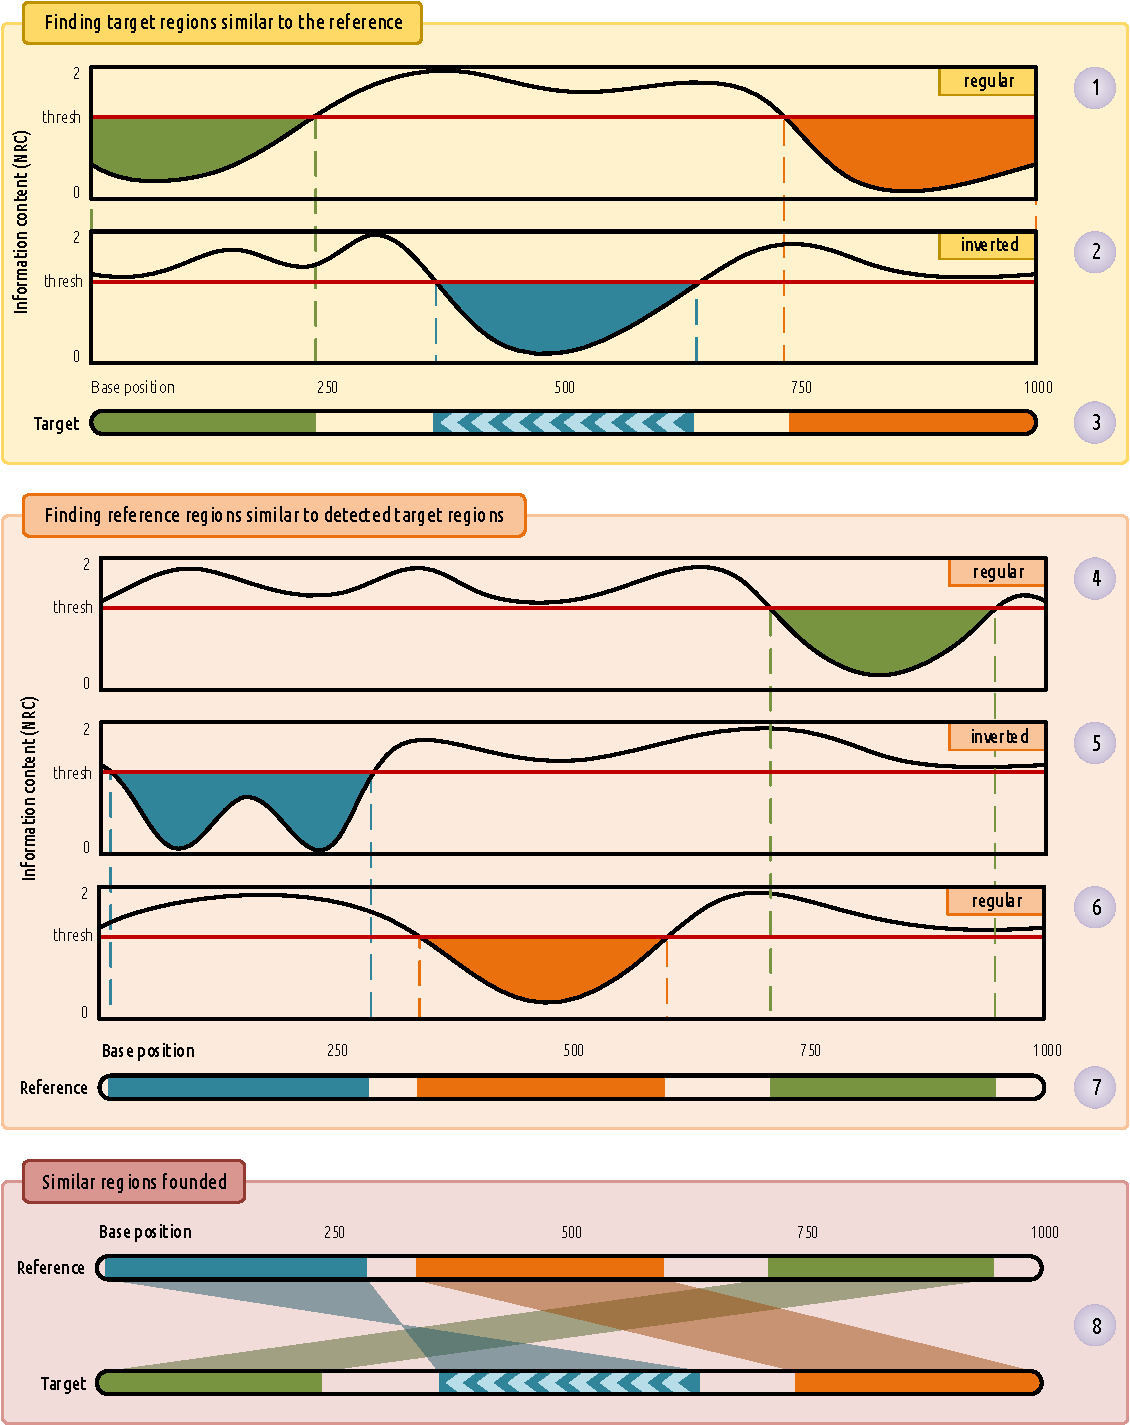
\includegraphics[width=\columnwidth]{simil.pdf}
   \caption{Finding similar regions in reference and target sequences. Smash++ finds, first, the regions in the target that are similar to the reference, and then, finds the regions in the reference that are similar to the detected target regions. This procedure is performance for both regular and inverted homologies.}
   \label{fig.simil}
 \end{figure}

 \subsection{Computing complexity}
 After finding the similar regions in reference and target sequences, we evaluate redundancy in each region, knowing that it is inversely related to Kolmogorov complexity, i.e., the more complex a sequence is, the less redundant it will be~\cite{hosseini2018cryfa}. The Kolmogorov complexity, $K$, of a binary string $s$, of finite length, is the length of the smallest binary program $p$ that computes $s$ in a universal Turing machine and halts. In other words, $K(s)=|p|$ is the minimum number of bits required to computationally retrieve the string $s$~\cite{turing1936on,li2009an}.

 The Kolmogorov complexity is not computable, hence, an alternative is required to compute it approximately. It has been shown in the literature that a compression algorithm can be employed for this purpose~\cite{zenil2015two,antao2018kolmogorov,faloutsos2007on}. In this paper, we employ a reference-free compressor to approximate the complexity and consequently, the redundancy of the founded similar regions in the reference and the target sequences. This compressor works based on cooperation of FCMs and STMMs, which has been previously described in detail. Note that the difference between reference-based and reference-free version of such compressor is that in the former mode, a model is first created for the reference sequence and then, the target sequence is compressed based on that model, while in the latter mode, the model is progressively created at the time of compressing the target sequence.


\section{Experiments setup} \label{sec.experiment}


\subsection{Datasets}

\begin{table*}[h]
  \caption{Datasets used in the experiments.}
  \label{tab.dataset}
  \begin{tabularx}{\linewidth}{lrlrX}
    \toprule
    Reference & \multicolumn{1}{l}{Length (base)} & Target & \multicolumn{1}{l}{Length (base)} & Description \\
    \midrule
    \multicolumn{5}{l}{Synthetic data -- generated by GOOSE toolkit\textsuperscript{*}} \\
    \midrule
    RefS & 1,000 & TarS & 1,000 &  RefS consists of four segments of size~250 bases. To build TarS, segments~I and IV are inversely repeated, II is mutated~1\% and III is duplicated. Read lines are 50~base long. \\
    RefM & 100,000 & TarM & 100,000 & For building TarM, segments~I and III of RefM (out of total~four) are duplicated, II is inversely repeated and IV is mutated~1\%. The length of read lines is 100. \\
    RefL & 5,000,000 & TarL & 5,000,000 & RefL includes four segments, 1,250,000~bases each. Segments~I and III are duplicated, II is mutated~1\% and IV is inversely repeated for building TarL. Read lines are of length 100~bases. \\
    RefXL & 100,000,000 & TarXL & 100,000,000 & RefXL is made of four segments, 25,000,000~bases each. Segment~I is mutated~1\%, segments~II and III are inversely repeated and segment~IV is duplicated to make TarXL. Read lines are 100~base long. \\
    RefMut & 60,000 & TarMut & 60,000 & RefMut includes 60 segments. To build TarMut, the first segment~(I) is mutated~1\%, the second segment is mutated~2\%, the third one is mutated~3\%, and so on. The length of read lines is 100. \\
    \midrule
    Real data \\
    \midrule
    \bottomrule
  \end{tabularx}
  
\begin{tablenotes}
\item \textsuperscript{*}\url{https://github.com/pratas/goose}
\end{tablenotes}
\end{table*}

\section{Results} \label{sec.results}
Smash++ and several other methods have been carried out on a collection of synthetic and real sequences. The machine used for the tests had an 8-core 3.40~GHz Intel\textsuperscript{\textregistered} Core{\texttrademark} i7-6700 CPU and 32~GB of RAM.

\begin{figure*}[!h]
  \centering
  \includegraphics[width=\linewidth]{synth.pdf}
  \caption{synthetic.}
  \label{fig.synth}
\end{figure*}





% The methods section should include the design of the study, the type of materials involved, a clear description of all comparisons, and the type of analysis used, to enable replication of the work. Ease of reproducibility is one of the key criteria on which reviewers will be asked to comment, so we strongly advocate the use of the reporting checklists recommended by the \href{https://biosharing.org/}{BioSharing} network and workflow management systems such as \href{https:/galaxyproject.org/}{Galaxy} and \href{http://www.myexperiment.org/home}{MyExperiment} and container systems such as \href{https://www.docker.com/}{Docker}, to save the details of the methods to encourage reproducibility as well as conciseness, is also strongly encouraged. Our \href{http://gigadb.org/}{\textit{Giga}DB repository}{} and \href{http://galaxy.cbiit.cuhk.edu.hk/}{GigaGalaxy} server can also be used to archive data, workflows and snapshots of the code with an accompanying DOI. Our \href{https://github.com/gigascience/papers}{GitHub page} can also be used to host a dynamic forkable version of the code if the authors have not used a code repository themselves.

% \emph{GigaScience} encourages and assists with the submission of detailed protocols to the open access repository \href{https://www.protocols.io/}{protocols.io}. Please enter the details into protocols.io, issue a DOI, and cite the protocols.io record from the Methods section.

% Authors benefit greatly by posting their methods in protocols.io as these are in a formatted form, allow inclusion of all the details, are fully searchable unlike supplementary files, and can be updated to new versions as basic methodology changes over time. Doing this saves authors extensive time in the future as the methods do not need to be rewritten in future manuscripts as they need only be cited.

\section{Availability of source code and requirements (optional, if code is present)}

Lists the following:
\begin{itemize}
\item Project name: e.g.~My bioinformatics project
\item Project home page: e.g.~\url{http://sourceforge.net/projects/mged}
\item Operating system(s): e.g.~Platform independent
\item Programming language: e.g.~Java
\item Other requirements: e.g.~Java 1.3.1 or higher, Tomcat 4.0 or higher
\item License: e.g.~GNU GPL, FreeBSD etc.
Any restrictions to use by non-academics: e.g. licence needed
\end{itemize}

This needs to be under an \href{http:/opensource.org/licenses}{Open Source Initiative} approved license where practicable compiled running software is made available. If the code is not hosted in a repository the \href{https://github.com/gigascience}{\textit{GigaScience} GitHub repository} is also available for this purpose.

\section{Availability of supporting data and materials}

\textit{GigaScience} requires authors to deposit the data set(s) supporting the results reported in submitted manuscripts in a publicly-accessible data repository such as \href{http://gigadb.org/}{\textit{Giga}DB} (see \textit{Giga}DB database terms of use for complete details). This section should be included when supporting data are available and must include the name of the repository and the permanent identifier or accession number and persistent hyperlinks for the data sets (if appropriate). The following format is recommended:

``The data set(s) supporting the results of this article is(are) available in the [repository name] repository, [cite unique persistent identifier].''

Following the \href{https://www.force11.org/group/joint-declaration-data-citation-principles-final}{Joint Declaration of Data Citation Principles}, where appropriate we ask that the data sets be cited where it is first mentioned in the manuscript, and included in the reference list. If a DOI has been issued to a dataset please always cite it using the DOI rather than the less stable URL the DOI resolves to (e.g.~\url{http://dx.doi.org/10.5524/100044} rather than \url{http://gigadb.org/dataset/100044}). For more see:

Data Citation Synthesis Group: Joint Declaration of Data Citation Principles. Martone M. (ed.) San Diego CA: FORCE11; 2014 [\url{https://www.force11.org/datacitation}]

A list of available scientific research data repositories can be found in \href{http://www.re3data.org/}{res3data} and \href{https://biosharing.org/}{BioSharing}.

\section{Declarations}

\subsection{List of abbreviations}
CMLS: Count-Min-Log Sketch; CPU: central processing unit; FCM: finite-context model; GB: gigabyte; GHz: gigahertz; KB: kilobyte; MB: megabyte; RAM: random access memory; PRNG: pseudo-random number generator; STMM: substitutional tolerant Markov model.

\subsection{Ethical Approval (optional)}
Manuscripts reporting studies involving human participants, human data or human tissue must:

\begin{itemize}
\item include a statement on ethics approval and consent (even where the need for approval was waived)
\item include the name of the ethics committee that approved the study and the committee's reference number if appropriate
\end{itemize}

Studies involving animals must include a statement on ethics approval and have been treated in a humane manner in line with the \href{http://www.nc3rs.org.uk/arrive-guidelines}{ARRIVE guidelines}.

See our \href{https://academic.oup.com/gigascience/pages/editorial_policies_and_reporting_standards}{editorial policies} for more information.

If your manuscript does not report on or involve the use of any animal or human data or tissue, this section is not applicable to your submission. Please state ``Not applicable'' in this section.

\subsection{Consent for publication}

If your manuscript contains any individual person's data in any form, consent to publish must be obtained from that person, or in the case of children, their parent or legal guardian. All presentations of case reports must have consent to publish. You can use your institutional consent form. You should not send the form to us on submission, but we may request to see a copy at any stage (including after publication). Please also confirm you have followed national guidelines on data collection and release in the place the research was carried out, for example confirming you have Ministry of Science and Technology (MOST) approval in China.

If your manuscript does not contain any individual person's data, please state ``Not applicable'' in this section.

\subsection{Competing Interests}
The authors declare that they have no competing interests.


\subsection{Funding}
This work was supported by Programa Operacional Factores de Competitividade -- COMPETE (FEDER); and by national funds through the Foundation for Science and Technology (FCT), in the context of the projects [UID/CEC/00127/2013, PTCD/EEI-SII/6608/2014] and the grant [PD/BD/113969/2015].


\subsection{Author's Contributions}

The individual contributions of authors to the manuscript should be specified in this section. Guidance and criteria for authorship can be found in our \href{https://academic.oup.com/gigascience/pages/editorial_policies_and_reporting_standards}{editorial policies}. We would recommend you follow some kind of standardised taxonomy like the \href{http://docs.casrai.org/CRediT}{CASRAI CRediT} (Contributor Roles Taxonomy).


\section{Acknowledgements}

Please acknowledge anyone who contributed towards the article who does not meet the criteria for authorship including anyone who provided professional writing services or materials.

Authors should obtain permission to acknowledge from all those mentioned in the Acknowledgements section. If you do not have anyone to acknowledge, please write ``Not applicable'' in this section.

See our \href{https://academic.oup.com/gigascience/pages/editorial_policies_and_reporting_standards}{editorial policies} for a full explanation of acknowledgements and authorship criteria.

Group authorship: if you would like the names of the individual members of a collaboration group to be searchable through their individual PubMed records, please ensure that the title of the collaboration group is included on the title page and in the submission system and also include collaborating author names as the last paragraph of the “Acknowledgements” section. Please add authors in the format First Name, Middle initial(s) (optional), Last Name. You can add institution or country information for each author if you wish, but this should be consistent across all authors.

Please note that individual names may not be present in the PubMed record at the time a published article is initially included in PubMed as it takes PubMed additional time to code this information.

\section{Authors' information (optional)}

You may choose to use this section to include any relevant information about the author(s) that may aid the reader's interpretation of the article, and understand the standpoint of the author(s). This may include details about the authors' qualifications, current positions they hold at institutions or societies, or any other relevant background information. Please refer to authors using their initials. Note this section should not be used to describe any competing interests.



%% Specify your .bib file name here, without the extension
\bibliography{paper-refs}

% \begin{landscape}
% \begin{table}
% \caption{Automobile land speed records (GR 5-10). This is again the same table as before, but on a landscaped page. \textbf{Note that a hard page break is inserted immediately before and after \texttt{landscape}}, so you'll need to carefully position such an environment at a suitable location in your manuscript!}
% \label{tab:example:landscape}
% \begin{tabularx}{\linewidth}{S l l l r L}
% \toprule
% {Speed (mph)} & {Driver} & {Car} & {Engine} & {Date} & {Extra comments}\\
% \midrule
% 407.447     & Craig Breedlove & Spirit of America          & GE J47    & 8/5/63  & (Just to demo a full-width table with auto-wrapping long lines) \\
% 413.199     & Tom Green       & Wingfoot Express           & WE J46    & 10/2/64  \\
% 434.22      & Art Arfons      & Green Monster              & GE J79    & 10/5/64  \\
% 468.719     & Craig Breedlove & Spirit of America          & GE J79    & 10/13/64 \\
% 526.277     & Craig Breedlove & Spirit of America          & GE J79    & 10/15/65 \\
% 536.712     & Art Arfons      & Green Monster              & GE J79    & 10/27/65 \\
% 555.127     & Craig Breedlove & Spirit of America, Sonic 1 & GE J79    & 11/2/65  \\
% 576.553     & Art Arfons      & Green Monster              & GE J79    & 11/7/65  \\
% 600.601     & Craig Breedlove & Spirit of America, Sonic 1 & GE J79    & 11/15/65 \\
% 622.407     & Gary Gabelich   & Blue Flame                 & Rocket    & 10/23/70 \\
% 633.468     & Richard Noble   & Thrust 2                   & RR RG 146 & 10/4/83  \\
% 763.035     & Andy Green      & Thrust SSC                 & RR Spey   & 10/15/97\\
% \bottomrule
% \end{tabularx}

% \begin{tablenotes}
% \item Source is from this website: \url{https://www.sedl.org/afterschool/toolkits/science/pdf/ast_sci_data_tables_sample.pdf}
% \end{tablenotes}
% \end{table}
% \end{landscape}



\end{document}
